\chapter{Interactions in Proteins}

\begin{introduction}
    \item 
\end{introduction}

\hypertarget{basic-concepts}{%
	\section{Basic concepts}\label{basic-concepts}}

Internal energy involves:

\begin{itemize}
	\item
	kinetic energy
	\item
	potential energy
\end{itemize}

Recall three thermodynamical laws.

\begin{emptytcb*}{To roughly remember}{}
	Life is but a interplay of weak forces (non-bonding interactions)
	\begin{longtable}[]{@{}ll@{}}
		\toprule
		bond & energy (\(\mathrm{kJ/mol}\))\tabularnewline
		\midrule
		\endhead
		ionic (\(\ce{COO-}\) and \(\ce{NH3+}\)) &
		20\textasciitilde{}80\tabularnewline
		hydrogen & 4\textasciitilde{}50, depending on distance and
		orientation\tabularnewline
		dipole (\(\ce{CO}\) and \(\ce{CO)}\) & 5\textasciitilde{}10\tabularnewline
		vdw & 0.5\textasciitilde{}3 per atom pair\tabularnewline
		hydrophobic & 4\textasciitilde{}8 per non-polar groups\tabularnewline
		\bottomrule
	\end{longtable}
	
	Functions of non-bonding interactions:
	
	\begin{itemize}
		\item
		additional strength to stabilize (high level structure)
		\item
		flexible, interact and perform functions
	\end{itemize}
\end{emptytcb*}

\hypertarget{general-electrostatic-interactions}{%
	\section{General electrostatic
		interactions}\label{general-electrostatic-interactions}}

\hypertarget{ion-ion}{%
	\subsection{ion-ion}\label{ion-ion}}

For atoms carrying charge.

\begin{itemize}
	\item
	equation
	
	\[V=\dfrac{Q_iQ_j}{4\pi\varepsilon_0\varepsilon_rr_{ij}}\]
	
	\begin{itemize}
		\item
		\(\varepsilon_r\) : relative dielectric constant
		\item
		The force is weaker in water (larger \(\varepsilon_r=78.5\)) than in
		hydrophobic core (though hard to measure)/other organic solvents.
	\end{itemize}
	\item
	salt effect
	
	\begin{gather*}
	I=\dfrac{1}{2}\sum c_iq_i^2\\
	D=\sqrt{\dfrac{\varepsilon_0\varepsilon_rk_BT}{2N_Ae^2I}}\\
	V=\dfrac{Q_iQ_j}{4\pi\varepsilon_0\varepsilon_r}\dfrac{\exp(-r_{ij}/D)}{r_{ij}}
	\end{gather*}
	
	\(I \uparrow,\ V\downarrow\). "Neutralizing charges"
\end{itemize}

eg: N and C terminal, side chain (salt bridge)

\hypertarget{ion-dipole}{%
	\subsection{ion-dipole}\label{ion-dipole}}

\begin{itemize}
	\item
	for ion with groups carrying \underline{no formal charge}
	\item
	dipole: \textbf{negative \(\rightarrow\) positive} point charge
	\item
	dipolar molecule: those with dipole moment (\(\ce{H2O, CO}\))
\end{itemize}

\begin{figure}
	\centering
	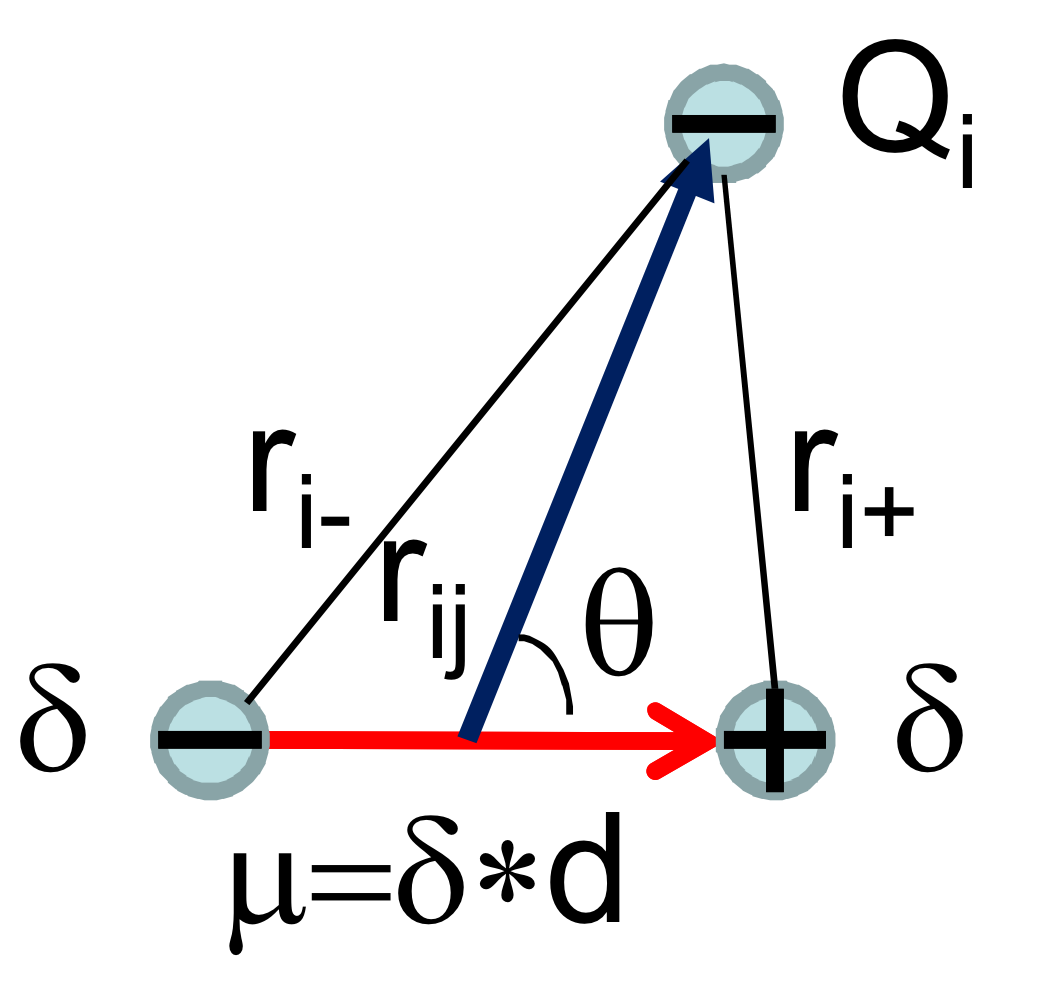
\includegraphics[width=0.3\linewidth]{E:/undergraduate_study/study/abroad study/2021 NUS/study/LSM3243/notes/2_1.png}
%	\caption{2\_1}
\end{figure}
\[V=\dfrac{Q_i\delta}{4\pi\varepsilon_0\varepsilon_r}(\dfrac{1}{r_{i-}}-\dfrac{1}{r_{i+}})=\dfrac{Q_i\delta}{4\pi\varepsilon_0\varepsilon_r}\cdot\dfrac{r_{i+}-r_{i-}}{r_{i-}r_{i+}}\approx\dfrac{Q_i\mu}{4\pi\varepsilon_0\varepsilon_rr_{ij}^2}\]

eg: disolve salt. \(\Delta H=E_{lattice}-E_{hydration}\), hydration: ion
with water.

entropy may increase.

\hypertarget{dipole-dipole}{%
	\subsection{dipole-dipole}\label{dipole-dipole}}

\begin{figure}
	\centering
	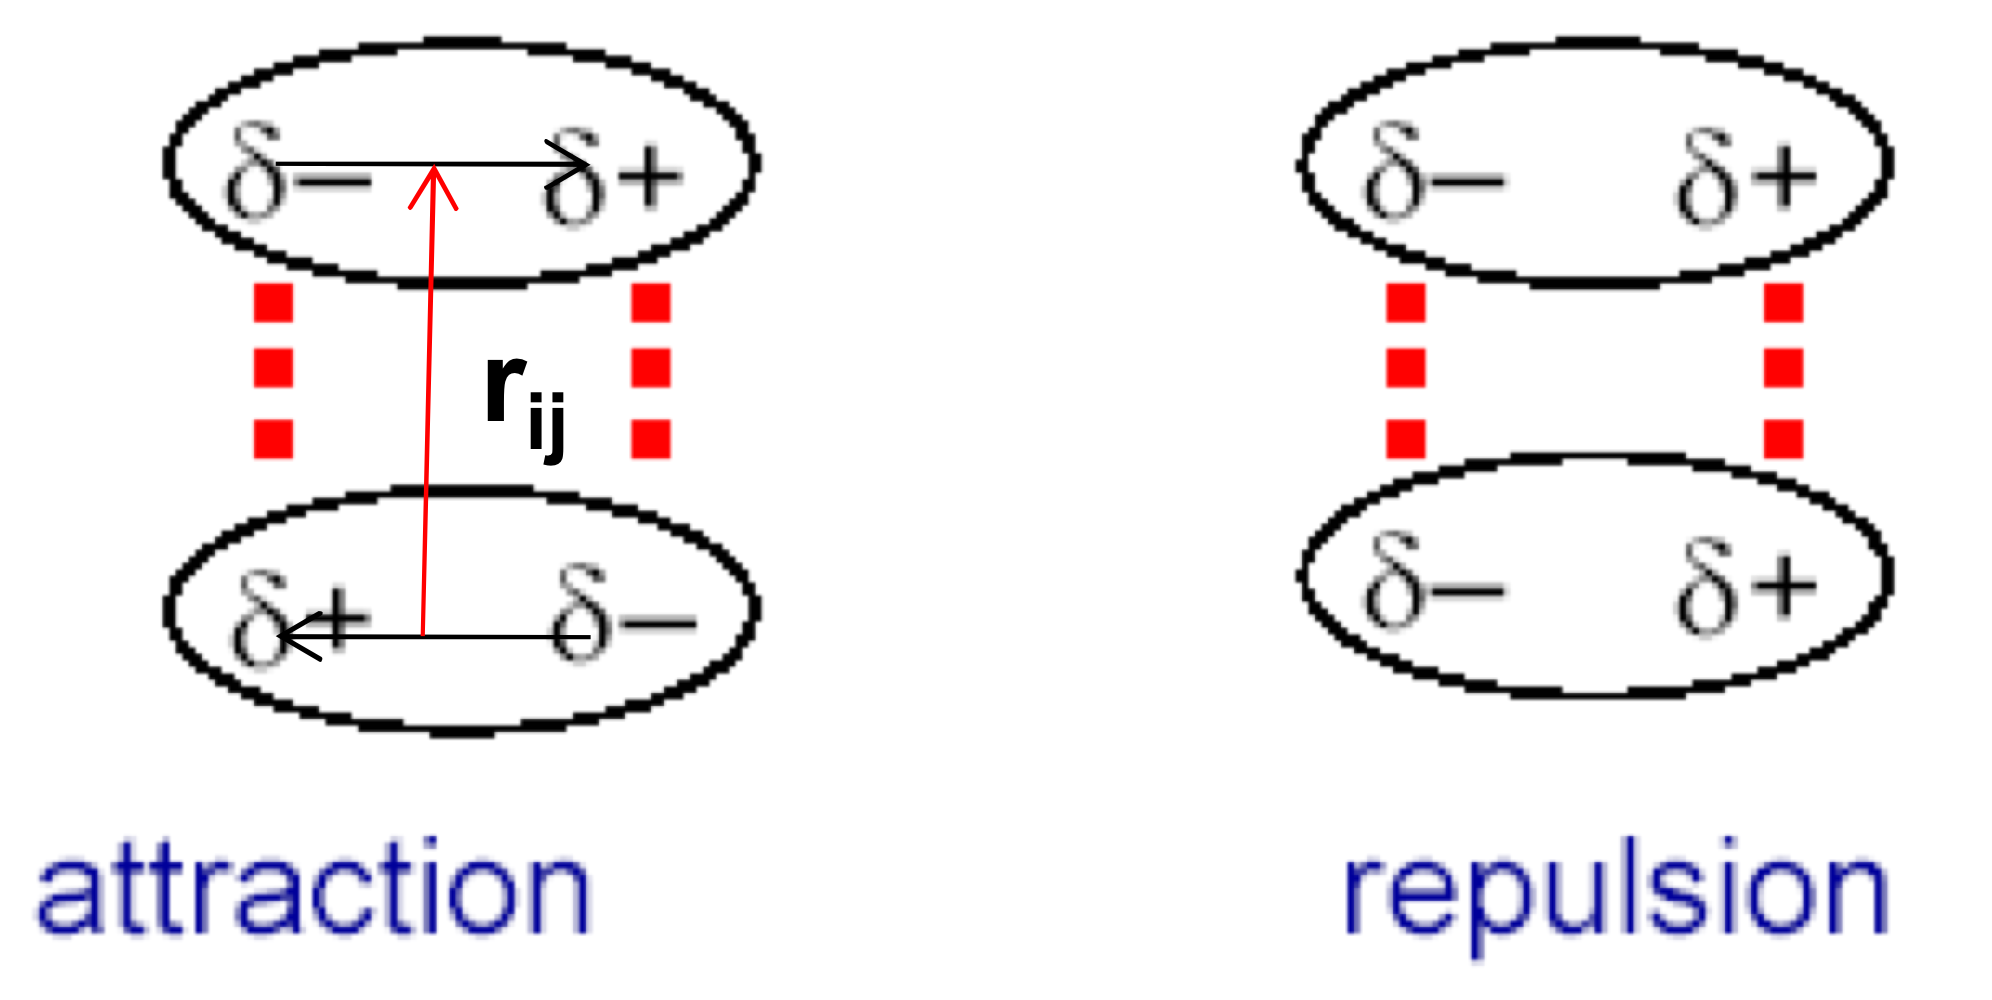
\includegraphics[width=0.5\linewidth]{E:/undergraduate_study/study/abroad study/2021 NUS/study/LSM3243/notes/2_2.png}
%	\caption{2\_2}
\end{figure}

\[V=\dfrac{1}{4\pi\varepsilon_0\varepsilon_r}\left[\dfrac{\mu_i\cdot\mu_j}{r_{ij}^3}-\dfrac{3(\mu_i\cdot r_{ij})\cdot(\mu_j\cdot r_{ij})}{r_{ij}^5}\right]\]

The potential depends on the relative orientation. The system tends to
lower the energy.

eg:

\begin{itemize}
	\item
	d-d interaction: \(\ce{H2O}>\ce{HCl}\)
	\item
	interaction between \(\alpha\) helices (accumulation of peptide bond
	polarity), important for attracting charged molecules and enhances
	reactions.
\end{itemize}

\hypertarget{van-der-waals}{%
	\section{van der Waals}\label{van-der-waals}}

here refers to dispersion forces

\begin{itemize}
	\item
	features
	
	\begin{itemize}
		\item
		temporary dipole, induced non-uniform e\textsuperscript{-}
		distribution
		\item
		contact distance, L-J potential
	\end{itemize}
	\item
	important for molecules both with and without permanent dipoles
	\item
	significant for large molecules
\end{itemize}

\hypertarget{hydrogen-bond-1}{%
	\section{hydrogen bond}\label{hydrogen-bond-1}}

\begin{figure}
	\centering
	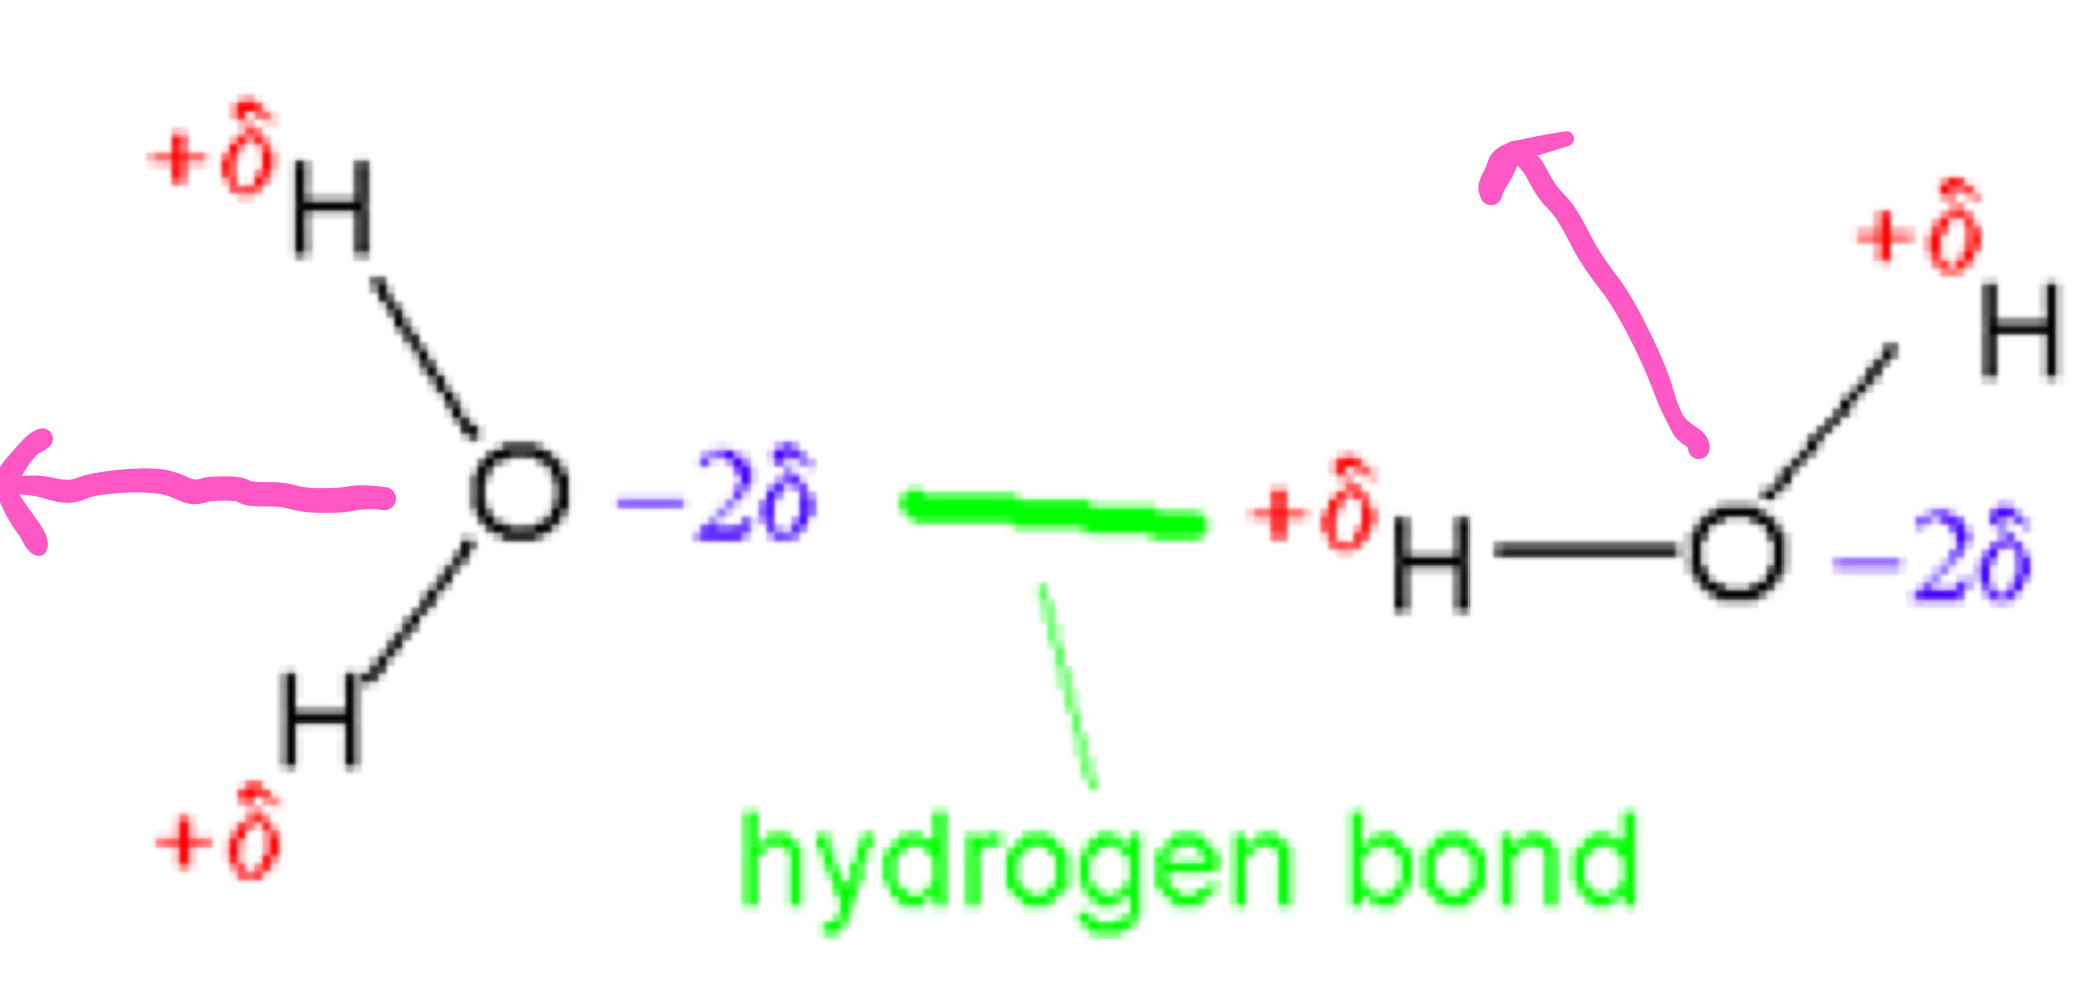
\includegraphics[width=0.5\linewidth]{E:/undergraduate_study/study/abroad study/2021 NUS/study/LSM3243/notes/2_5.png}
%	\caption{2\_5}
\end{figure}

\begin{itemize}
	\item
	features
	
	\begin{itemize}
		\item
		short range: \(r_{bond}\ll r<R_{vdw}\)
		\item
		directionality: 120\textasciitilde{}180°
	\end{itemize}
	\item
	affects secondary structure \& recognition, but not
	dominating/determining folding/assembly
	\item
	only intramolecular H bonds in the interior of a protein are favorable
	in presence of competition from water
\end{itemize}

actually vdW and H bond are both special cases of dipole-dipole
interaction

\hypertarget{hydrophobic-interaction}{%
	\section{hydrophobic interaction}\label{hydrophobic-interaction}}

Oil doesn't mix with water. The molecules attract themselves more than
each other. Thus mixing water and oil is only a process where water
molecules form a cage (more ordered, to strengthen interaction) rather
than thorough mixing.

Their attraction increases (\(\Delta H<0\)) but the deterministic factor
is \(\Delta S(\ce{H2O})<0\). To minimize the entropy decrease,
hydrophobic parts tend to gather to make their volume lowest and water
molecules to form a cage least.

\begin{figure}
	\centering
	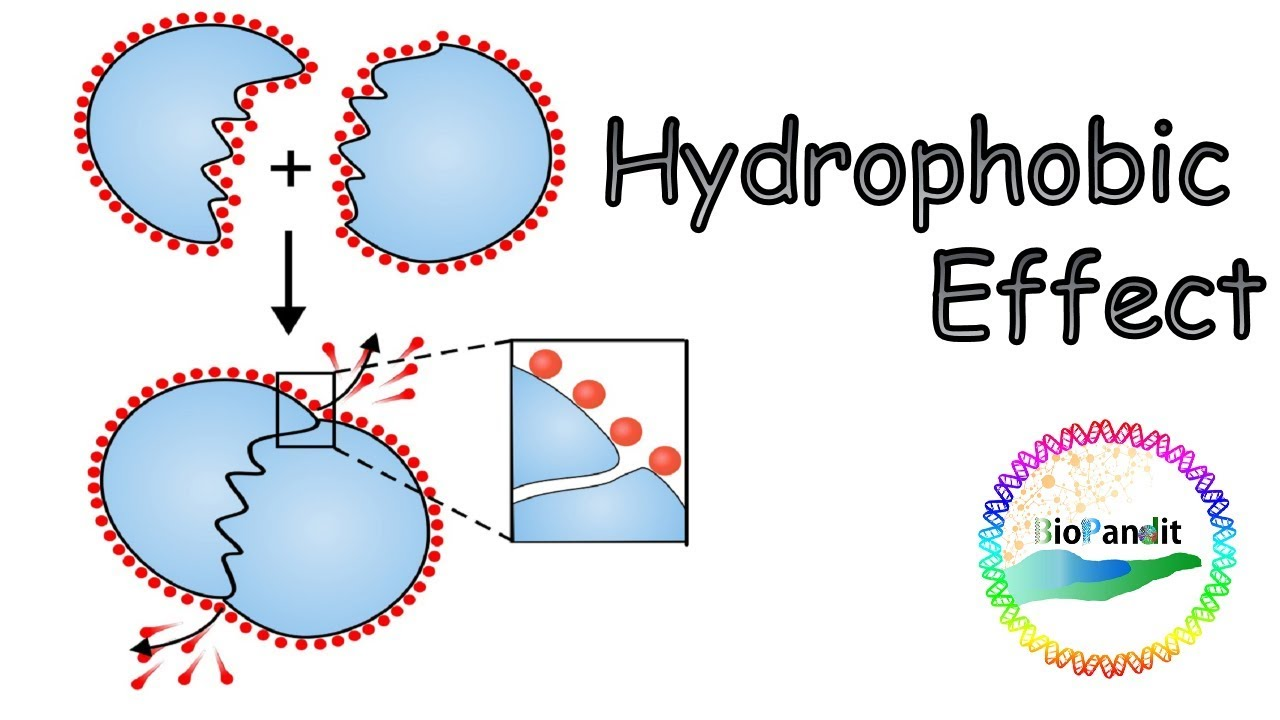
\includegraphics[width=0.7\linewidth]{E:/undergraduate_study/study/abroad study/2021 NUS/study/LSM3243/notes/2_6.jpg}
%	\caption{2\_6}
\end{figure}

\hypertarget{disulfide-bonds}{%
	\section{Disulfide bonds}\label{disulfide-bonds}}

Fold first, then disulfide bonds!